\section{Depth-First Search (DFS) (Tiefensuche)}

\subsection{Definition}
\begin{itemize}
    \item ist allgemeine Technik für die Traversierung eines Graphen
    \item Eine DFS Traversierung eines Graphen G
    \begin{itemize}
        \item besucht alle Vertizes und Kanten von G
        \item bestimmt, ob G verbunden ist
        \item berechnet / bestimmt die verbundenen Komponenten von G
        \item berechnet einen aufspannenden Wald von G
    \end{itemize}
    \item DFS kann man auch erweitern, um andere Graphenprobleme zu lösen
    \item Depth-First Search entspricht in etwa der Euler-Tour bei binären Bäumen
\end{itemize}


\subsection{Laufzeit}
\begin{itemize}
    \item DFS auf einem Graphen mit n Vertizes und m Kanten benötigt O(n + m) Zeit
    \item Setzen/Lesen eines Vertex-/Kanten-Labels benötigt O(1) Zeit
    \item Jeder Vertex wird zweimal markiert:
    \begin{itemize}
        \item zuerst als UNEXPLORED
        \item dann als VISITED
    \end{itemize}
    \item Jede Kante wird zweimal markiert:
    \begin{itemize}
        \item zuerst als UNEXPLORED
        \item dann als DISCOVERY oder BACK
    \end{itemize}
    \item Die Methode incidentEdges() wird pro Vertex einmal aufgerufen
\end{itemize}


\subsection{Algorithmus}
\begin{center}
    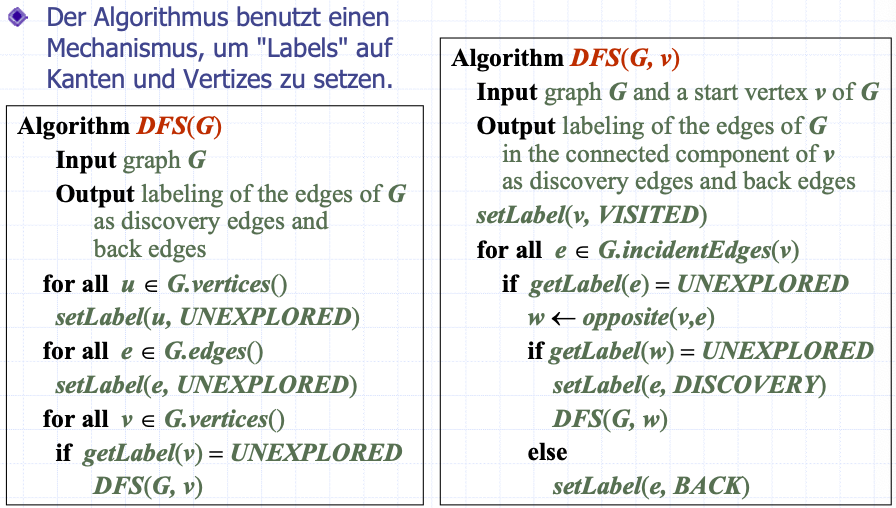
\includegraphics[scale=.4]{graphic/12 DFS/Algorithmus.png}
\end{center}
\vspace{-8pt}


\subsection{Beispiel}
\begin{center}
    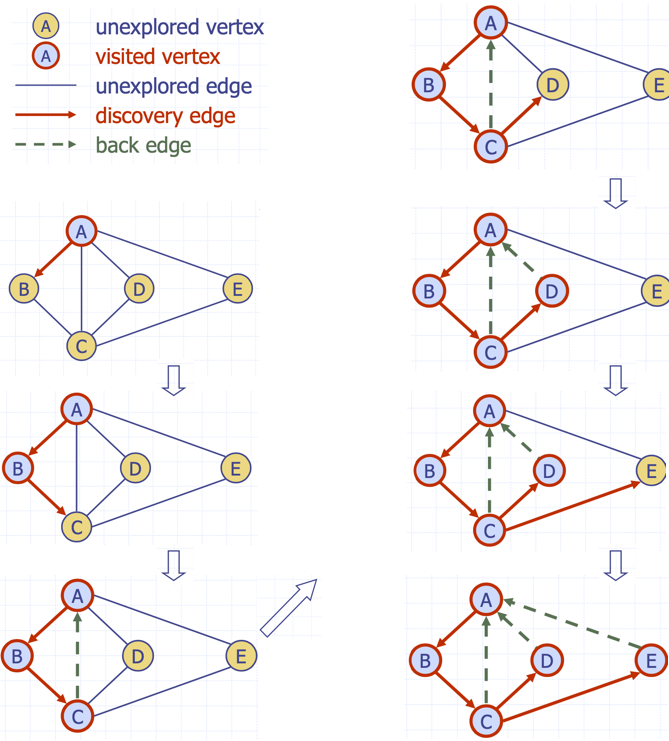
\includegraphics[scale=.4]{graphic/12 DFS/Beispiel.png}
\end{center}
\vspace{-8pt}


\subsection{Labyrinth}
Der DFS Algorithmus ähnelt der klassischen Strategie zur Erkundung eines Labyrinths:
\begin{itemize}
    \item markieren jede besuchte Kreuzung, Ecke und Sackgasse (Vertex)
    \item wir markieren jeden besuchten Korridor (Kante)
    \item notieren den Rückweg zum Eingang (Start Vertex) ($\rightarrow$ Rekursion auf dem Stack)
\end{itemize}


\subsection{Eigenschaften}
\begin{itemize}
    \item \textbf{Eigenschaft 1:} DFS(G, v) besucht alle Vertizes und Kanten in der verbundenen Komponente von G beginnend bei v
    \item \textbf{Eigenschaft 2:} die von DFS(G, v) markierten, besuchten Kanten bilden einen aufspannenden Baum für die verbundene Komponente von G beginnend bei v
\end{itemize}

\subsection{Pfade finden}
\begin{itemize}
    \item DFS Algorithmus spezialisieren, um einen Pfad zwischen zwei gegebenen Vertizes u und z zu finden.
    \item zuerst DFS(G, u) aufrufen mit u als Startvertex
    \item mithilfe eines Stacks S den Pfad merken zwischen dem Startvertex und dem aktuellen Vertex
    \item sobald Zielvertex z gefunden, Pfad mithilfe des Stacks ausgeben
\end{itemize}
\vspace{-8pt}
\begin{center}
    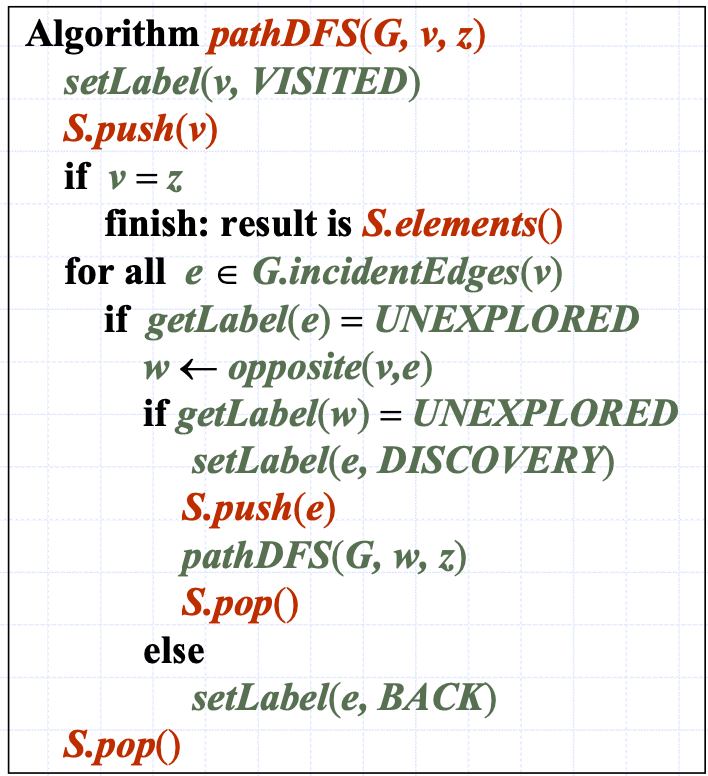
\includegraphics[scale=.3]{graphic/12 DFS/Pfade finden.png}
\end{center}
\vspace{-8pt}


\subsection{Zyklen finden}
\begin{itemize}
    \item DFS Algorithmus spezialisieren, um einfache Zyklen zu finden
    \item mithilfe eines Stacks S den Pfad merken zwischen Startvertex und aktuellen Vertex
    \item sobald auf eine Back- Edge (v, w) treffen, Zyklus als Teil des Stacks aus:
    \item vom obersten Stackelement bis zum Vertex w.
\end{itemize}
\vspace{-8pt}
\begin{center}
    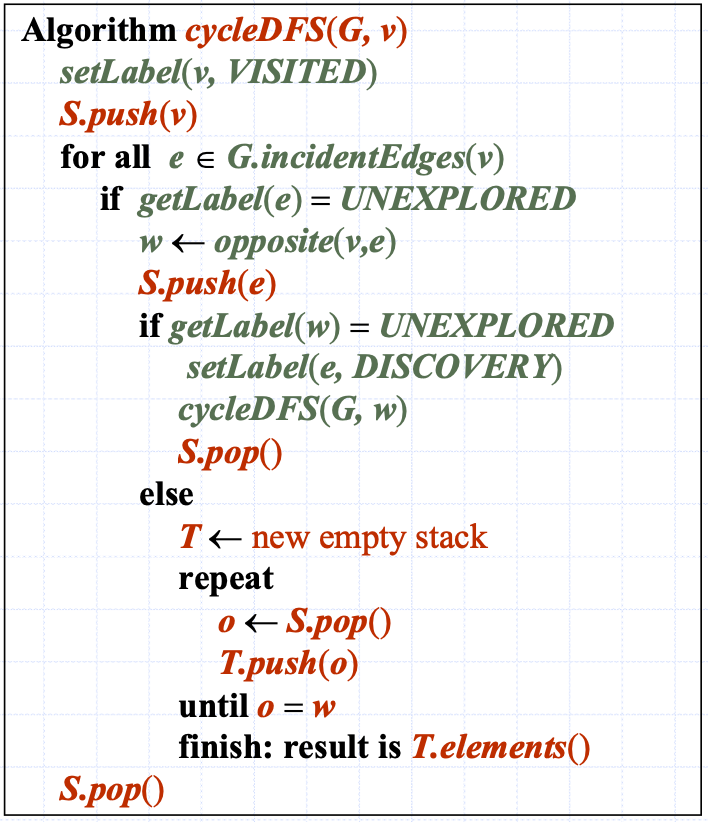
\includegraphics[scale=.3]{graphic/12 DFS/Zyklen finden.png}
\end{center}
\vspace{-8pt}

\vfill
$ $
\columnbreak
\paragraph{Tiefensuche}
\begin{center}
    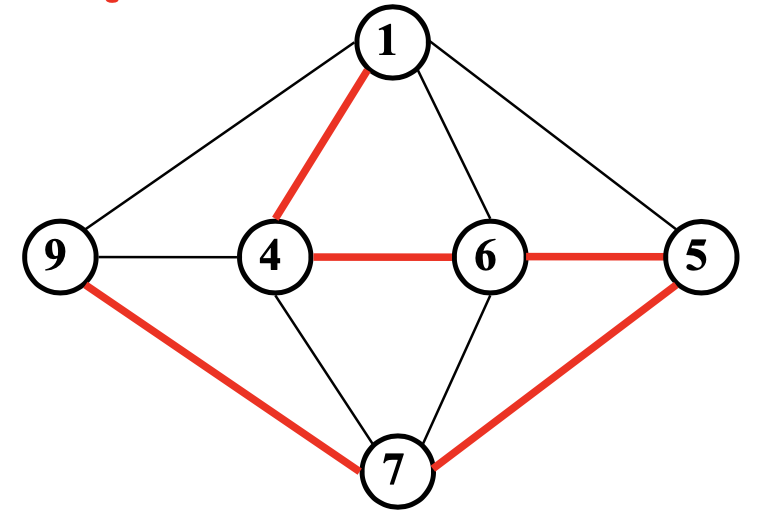
\includegraphics[scale=.3]{12 DFS/tiefensuche.png}
\end{center}

\paragraph{Gerichtete Tiefensuche Typen}
\begin{center}
    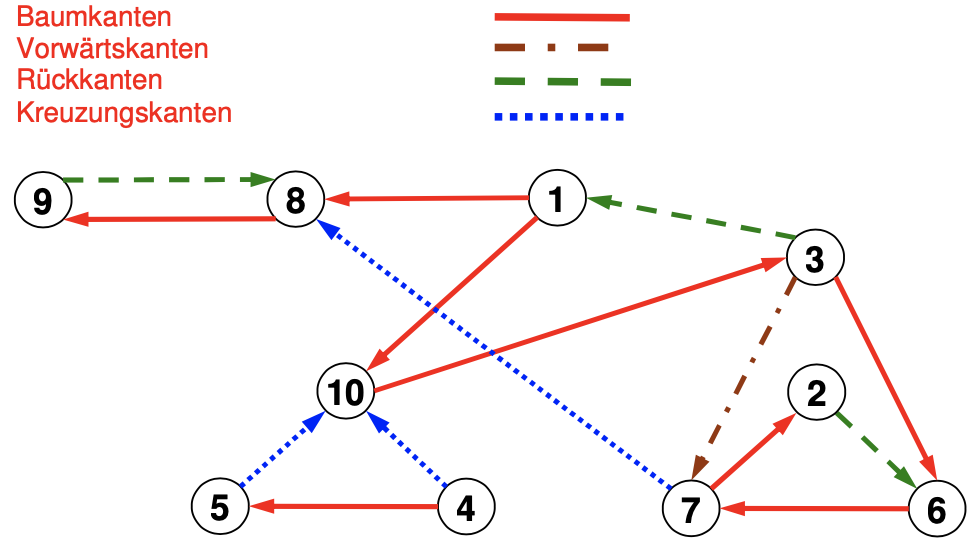
\includegraphics[scale=.33]{12 DFS/gerichtete_tiefensuche.png}
\end{center}


\paragraph{Gerichtete Tiefensuche Algorithmus}
\begin{enumerate}
    \item Starte bei 1 respektive A
    \item Gehe zum nächstliegenden Buchstaben / Zahl
    \item Solange in Tiefe suchen, bis nicht mehr weiter geht
    \item Zurück, bis wieder weitergesucht werden kann
\end{enumerate}
\begin{center}
    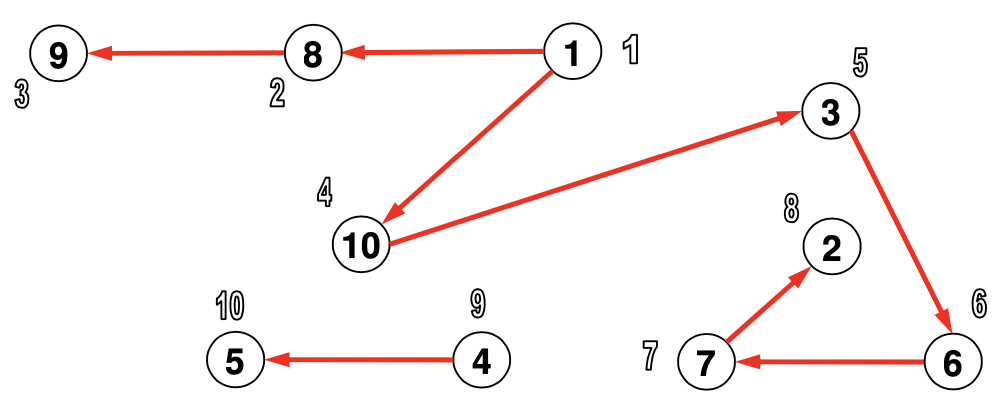
\includegraphics[scale=.33]{12 DFS/gerichtete_tiefensuche_alg.png}
\end{center}


\newpage